\documentclass[journal]{IEEEtran}

\renewcommand{\baselinestretch}{1.0} % Change to 1.65 for double spacing
 
\usepackage{amsmath,amsfonts,amssymb}
\usepackage{graphicx}
\usepackage[colorlinks=true, allcolors=blue]{hyperref}


\usepackage{color}
\usepackage[latin9]{inputenc}
\usepackage{mathrsfs,amsmath}
\usepackage{graphicx}%
\usepackage{float}
\usepackage{amsfonts}%
\usepackage{amssymb}
\usepackage{braket}
\usepackage{bm}
%necessary for outline section of the article 
\usepackage{outline}

\newcommand{\mb}[1]{\bm{#1}}
\usepackage[T1]{fontenc}

\def\Nabla{\bm{\nabla}}
\def\bm{\mathbf}
\def\curl{\Nabla\times}
\def\div{\Nabla\cdot}
\def\lap{\Delta}
\def\vlap{\Delta}
\def\x{\hat{e}_{x}}
\def\y{\hat{e}_{y}}
\def\z{\hat{e}_{z}}
\def\p{\partial}
\def\h{\hat}
\def\tw{\tilde{\omega}}
\def\gm{\gamma}
\def\om{\omega}
\def\OM{\Omega}
\def\GM{\Gamma}
\def\dw{\delta\omega}
\def\dth{\Delta\theta}
\def\dk{\delta k}
\def\Hdth{\frac{\dth}{2}} %half Delta Theta
\DeclareMathOperator{\Tr}{Tr}


\title{Analysis of operating regimes of terahertz quantum cascade laser frequency combs}
\author{\IEEEauthorblockN{Petar Tzenov\IEEEauthorrefmark{1},
		David Burghoff\IEEEauthorrefmark{2},
		Qing Hu\IEEEauthorrefmark{2}, 
		Christian Jirauschek\IEEEauthorrefmark{1}}
	
	\IEEEauthorblockA{\IEEEauthorrefmark{1}Institute for Nanoelectronics, Technical University of Munich, D-80333 Munich, Germany}
	
	\IEEEauthorblockA{\IEEEauthorrefmark{2}Department of Electrical Engineering and Computer Science, Research Laboratory of Electronics, Massachusetts Institute of Technology, Cambridge, Massachusetts 02139, USA}
	\thanks{Corresponding author: P. Tzenov (email: petar.tzenov@tum.de ).}}



\IEEEtitleabstractindextext
 
\begin{document} 
\maketitle

	

\begin{abstract}
REWRITE REWRITE REWRITE -> overlaps with previous publication
Quantum cascade lasers (QCLs) promise to be efficient, cheap and compact sources of frequency combs in the mid- and far-infrared portions of the electromagnetic spectrum. Experimental results have shown comb generation in the mid-infrared as well as, more recently, the terahertz based on free running QCLs. The community appears to collectively agree that high order nonlinear optical processes, such as four wave mixing, are the main mode proliferation mechanisms that contribute to comb formation. In contrast, it has been argued that group velocity dispersion (GVD) is the thorn in the design of frequency combs as it leads to pulse broadening and limits the full exploitation of the gain bandwidth of the material. In the terahertz regime, the two widest comb generating devices demonstrated so far, have shown a strong variation of the beatnote?s linewidth with changing injection current, thus indicating that they experience "comb" regimes of operation that cover only a fraction of the whole dynamic range of these lasers. Here we present results from a coupled ensemble Monte-Carlo (EMC) and Maxwell-Bloch (MB) equations simulations of a terahertz quantum cascade laser frequency comb.<-REWRITE REWRITE REWRITE 
\end{abstract}

\section{Introduction}
The Introduction serves to help the reader understand our
three key questions: Why is this a new and important problem?
What has been done before? How does your research bring
significant new understanding to the field? The reader should
find enough information to understand why your research was
necessary, without having to refer to other source material or
published works [7]. The introduction should be concise, no
more than one or two pages. It is written in the present tense.
Your introductory paragraph should start with what is generally
known about your subject. Then move step by step through
more detailed information, ending with a description of the
specific problem or hypothesis your article will discuss. Try to
use an attention-grabbing statement to hook the reader [10]
while being careful not to sensationalize your results.
In the next few paragraphs, refer to the published research to
show what is already known about your subject and why your
work is needed. Do not try to include everything from your
literature review. Your goal is to orient the reader to the most
relevant studies. Explain how each earlier study relates to your
own approach to the problem. Does it have limitations? Does it
make different assumptions [11]? Show your readers how your
study builds upon or is different from this existing work. If you
have published an earlier version of your work, for example as a
conference or journal article, you must explain how the current
study builds upon your own prior work [3].
After you have explained the historical context of your work,
introduce your hypothesis and provide a general description of
the results you have obtained. You will flesh these out more
fully later in the article, but providing an overview here motivates
your audience to read on. At the end of your introduction, tell
the reader how the article is organized. This will allow readers to
move to sections of particular interest, if they wish.

\section{Theoretical model}
\label{sec:theory}

Consider a prototypical THz QCL design, employing resonant tunneling for efficient current injection, schematically illustrated in Fig.~\ref{fig:basis}(a). In this configuration, the injector state is denoted as $\ket{1'}$, the upper laser level as $\ket{3}$ and the lower laser level as $\ket{2}$. Let us denote the tunneling coupling energy, as $\hslash\Omega_{1'3}$, the $1'\leftrightarrow 3$ detuning energy as $\hslash\epsilon$ and finally the energy of the optical, i.e. $3\leftrightarrow 2$, transition as $\hbar \omega_{32}$. The tunneling coupling between injector and upper laser level leads to a level splitting, i.e. the so called level anticrossing, of the states $\ket{1'}$ and $\ket{3}$ into a doublet of dressed states $\ket{+}$ and $\ket{-}$, which span the intramodule barrier, Fig.~\ref{fig:basis}(b), and have energy difference $\delta E = \hslash\sqrt{\epsilon^2 + 4\Omega_{1'3}^2}$.  

\begin{figure}[h!]
	\begin{center}
		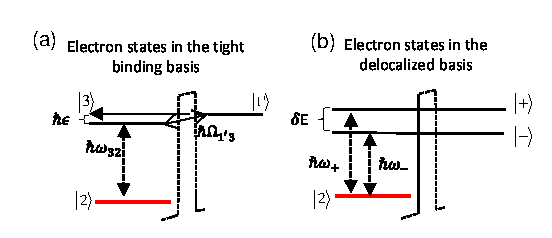
\includegraphics[width=0.45\textwidth]{IMGS/basis_compare2.eps}
		\caption{ (a) Schematic representation of a THz QCL design employing resonant tunneling injection, in the tight binding approximation. (b)  The eigenstates of the system in the delocalized basis, where the strong tunneling coupling between injector and upper lasers level leads to energy splitting into a pair of new eigenstates, $\ket{+}$ and $\ket{-}$.  The depopulation level as well as other laser levels are omitted from the diagram for brevity.} \label{fig:basis}
	\end{center}	
\end{figure}

The dipole coupling between the states $\ket{3}$ and $\ket{2}$ in the tight binding basis is transferred to a dipole interaction between both dressed states and $\ket{2}$, in essence producing a doublet of upper laser levels. If the anticrossing energy $\delta E$ is sufficiently large and the linewidth of the $\ket{3}\leftrightarrow\ket{2}$ transition is sufficiently narrow, this would lead to a splitting of the gain into a low and high frequency lobes, with angular frequencies $\omega_{-}$ and $\omega_{+}$, symmetrically distributed around $\omega_{32}$ \cite{dupont2010simplified}. Even though this extended basis picture is somewhat more intuitive, a density matrix treatment based on this approach has been shown to over-estimate the calculated current density and lead to erroneous predictions about the modelled device's performance \cite{callebaut2005importance}. This is due to the fact that in the delocalized basis picture of Fig.~\ref{fig:basis}(b), the electron transport through the barrier is immediate, since both $\ket{+}$ and $\ket{-}$ span the intramodule barrier, which therefore presents no resistance to the electron flow across the device. However, the presence of intrasubband, or pure, dephasing has been argued to lead to a build-up of electrons on the injector side of the barrier, which in turn leads to a decrease in the current density. Description of such an effect is most conveniently performed in the tight binding basis, which is why we will employ this formalism in our further theoretical treatment of the system. This allows us to treat the optical and tunneling couplings fully coherently via a density matrix approach, whereas all other scattering mechanisms, e.g. LO phonon, electron-electron, impurity and interface roughness scattering etc., phenomenologically as rate equations. \cite{kumar2009coherence}. 

Neglecting for the time being all phenomenological terms and including the interaction with the electric field within the electric dipole approximation, as well as the resonant tunneling coupling via the energy $\hslash\Omega_{1'3}$, the generator of time evolution of the system in Fig.~\ref{fig:basis}(a) is the following Hamiltonian operator, taken in the rotating wave approximation,
\begin{align}
\label{eq:hamiltonian-operatorform}
\h{H}^{\text{RWA}} &= \hbar(\epsilon + \Delta) \h\sigma_{1',1'} +\hbar\Delta\h\sigma_{3,3}  \nonumber \\ &+ (\hbar\Omega_{1'3}\h\sigma_{1',3} +\frac{q_0z_{32}}{2}f \h\sigma_{3,2}+H.c.).
\end{align}
In Eq. (\ref{eq:vonNeumann}) we have made the familiar ansatz decomposing the electric field $E_z(x,t) = \Re\{f(x,t) e^{i(k_0x-\omega_0t)}\}$ into the product of an envelope function $f(x,t)$ and a carrier wave with central angular frequency $\omega_0$ and wave number $k_0 = n\omega_0/c$. We have implicitly taken that the semiconductor growth direction of the QCL is along the z-axis and thus $E_z$ is the only component of the field coupling to the atomic system. Further, we have denoted with $n$ the background refractive index, with $c$ the velocity of light in vacuum and $z_{32} = \bra{3}\h{z}\ket{2} $ the dipole matrix element between states $\ket{3}$ and $\ket{2}$, where $\h{z}$ is the z-component of the position operator. $\Delta = \omega_{32} -\omega_0$ is the detuning of the electric field from $3\leftrightarrow 2$ resonance and we have set the zero energy to be equal to the energy of the lower level $E_2 = 0$. Finally, $\h \sigma_{i,j}$ denotes the atomic projection operators and "$H.c$" the Hermitian conjugate.

Within the Markovian approximation, the time evolution of the density operator $\h{\rho}^{\text{RWA}}$ is governed by the von Neumann equation with phenomenologically included dissipation term $G(\h{\rho}^{\text{RWA}})$ and is given by
\begin{equation}
\label{eq:vonNeumann}
\frac{d \h{\rho}^{\text{RWA}}}{dt} = -\frac{i}{\hbar}[\h{H}^{\text{RWA}};\h{\rho}^{\text{RWA}}] + G(\h{\rho}^{\text{RWA}}),
\end{equation}
where $[\cdot;\cdot]$ is the usual quantum mechanical commutator. Here the term $G(\h{\rho}^{\text{RWA}})$ is included to model the loss of coherence of the system due to interaction with the environment and is written within a standard scattering rates approach \cite{iotti2005microscopic}. Those rates are not taken as empirical values, but they were rather calculated with our ensemble Monte Carlo simulation code \cite{jirauschek2014modeling}, which incorporates all relevant incoherent scattering mechanisms for quantum cascade lasers \cite{jirauschek2009monte,jirauschek2010monte,jirauschek2010monte_2}.


In order to complete the description of the system, we simulate the time evolution of the forward and backward travelling components of the field envelope with the aid of a pair of propagation equations, and we also extend Eq. (\ref{eq:hamiltonian-operatorform}) accordingly,  to include  spatial hole burning (SHB) \cite{gordon2008multimode}, as well as the effect of additional laser levels from a single period of the active region. Since the resulting system of equations has been published elsewhere \cite{petz2016}, we omit further details on the technicalities, and instead focus our attention on the possible applications of our model for QCL device characterization. 

\section{Mode proliferation mechanisms}
\label{sec:proliferation}

Both theoretical \cite{khurgin2014coherent} and experimental \cite{friedli2013four} investigations have confirmed that four wave mixing (FWM), induced by the large third order non-linearity $\chi^{(3)}$, acts as the main mode-proliferation mechanism in free running mid- and far-infrared QCL devices.

For example, a series of pump-probe experiments were performed in Ref.~\cite{friedli2013four}, where a mid-IR QC amplifier was pumped with two single mode lasers, emitting a pair of frequencies, $f_1$ and $f_2$ (with $f_1 > f_2$), lying well under the gain spectrum of the device. Outcoupled light was consecutively recorded and subsequent spectral analysis revealed the clear footprints of degenerate four wave mixing, i.e. the generation of a pair of conjugate modes at the Stokes and anti-Stokes frequencies of  $f_s = 2f_2 -f_1 = f_2-\Delta f$ and $f_a = 2f_1 - f_2 = f_1+\Delta f$, respectively, where $\Delta f = f_1 - f_2$. Combined with the inherently broadband gain of QCLs, this effect could support the generation of more sidebands in a cascaded manner, ideally spanning the full bandwidth of the laser. Since FWM is an energy conserving process, in this way it ought to lead to an equidistant multimode spectrum and thus a frequency comb.

Unfortunately, this not always occurs due to the competition of FWM with various comb-degradation mechanisms such as group velocity dispersion (GVD) and multimode instabilities such as the Risken-Nummedal-Graham-Haken (RNGH) instability \cite{risken1968self,graham1968quantum}, argued to be with a lower threshold in QC lasers, due to spatial hole burning (SHB) \cite{gordon2008multimode}. From these the former, i.e. GVD, has been shown \cite{burghoff2015evaluating,villares2016dispersion} to play a major role in blocking the formation of a nice equidistantly-spaced spectrum. Therefore, state of the art QCL frequency combs usually employ sophisticated dispersion compensating mechanisms (DCMs), either based on a chirped corrugation structures embedded into the laser cavity \cite{burghoff2014terahertz} or GTI-mirrors positioned behind one of the facets of the laser \cite{villares2016dispersion}. Both techniques have shown to be very successful in eliminating the dispersion, leading to comb formation, there is still lack of understanding as to why lasers operating at negative GVD are easier to phase-lock \cite{villares2016dispersion} or why are the DCMs effective only within a narrow range from the overall operating regime \cite{burghoff2014terahertz}.

In order to understand in greater detail the various forms of interplay between FWM, GVD and SHB, we would need a robust theoretical model, capturing all of those effects with minimal restrictions on it's generality. For relatively narrow-band lasers, the slowly varying envelope (SVE) approximation allows the theoretical analysis of these processes within the framework of coupled ordinary differential equations for each of the lasing modes. Such an approach is limited, as it employs some stringent assumptions onto the spatio-temporal evolution of the modes, but nevertheless it has already been successfully employed for the investigation of the dominant comb-formation and comb-degradation mechanisms in QCLs \cite{khurgin2014coherent, villares2015quantum}.  

As a comparison, our model, briefly introduced in the previous section and in greater detail in Ref. \cite{petz2016}, still employs the SVE approximation, however it treats the propagation of the total electric field without imposing any assumptions on the spatial or temporal dependence of the modes. Even though this deprives us from obtaining robust analytical results, it nevertheless maintains the universality of the description, insofar as the SVE and the RWA approximations are justified, and allows us to simulate realistic QCL frequency comb devices. 

\begin{figure}[h!]
	\centering
	\includegraphics[width=0.40\textwidth]{IMGS/FWM_proof}
	\caption{(a) Optical spectrum obtained from THz-TDs simulations with two seed modes $f_1$ and $f_2$, separated by $\Delta f = 17.2$ GHz. The sidebands, detected at $f_s$ and $f_a$, with corresponding amplitudes $A_s$ and $A_a$, denote the FWM-generated Stokes and anti-Stokes waves. (b) same as (a) however the pump modes are separated by $\Delta f = 51.6$ GHz. (c) Dependence of the amplitudes of the sidebands, when the strength of the first pump at $f_1$ is varied, while $A_2$ is kept constant.  }	\label{fig:FWM_proof}
\end{figure}

Within our model, we can investigate the effect of different model parameters on the efficacy of FWM by essentially emulating laboratory experiments similar to those in Ref. \cite{friedli2013four}. Figures \ref{fig:FWM_proof}(a) and \ref{fig:FWM_proof}(b) show data from two such computations, when we simulated a laser, seeded through the left facet with two equally strong pump modes with frequencies $f_1$ and $f_2$, when we varied the mode spacing  $\Delta f = f_1 - f_2$. In both cases, the simulations were based on the THz QCL from Ref.~\cite{burghoff2014terahertz}, biased at 11 kV/cm. All scattering rates and other relevant active region parameters were calculated with the aid of our Schr�dinger-Possion and ensemble Monte Carlo codes~\cite{jirauschek2014modeling} and their values are not considerably different from the data published in Ref. \cite{petz2016}. Importantly, here we set the left and right amplitude reflectivities to only 5\%, in order to eliminate spatial hole burning from the simulation and thus isolate FWM as the only mode proliferation mechanism.

The logarithmic optical power spectrum clearly shows the emergence of signals at the Atokes and anti-Stokes frequencies only after 10 round trips of the light inside a simulated linear cavity of length $L = 2.5$ mm.  Based on the formalism in \cite{sutherland2003handbook}, we know that the amplitudes of the generated sidebands at $f_a$ and $f_s$ will experience the following dependence on the pump amplitudes, i.e. $A_{1}$ and $A_{2}$, and the nonlinear susceptibility $\chi^{(3)}$:
\begin{align}
A_{a} &\propto \chi^{(3)}(f_1,-f_2,f_1;-f_a) A_{1}^2 A_{2}, \nonumber \\
A_{s} &\propto \chi^{(3)}(-f_1,f_2,f_2;-f_s) A_{1}  A_{2}^2. \label{eq:susceptibility}
\end{align}

Figure \ref{fig:FWM_proof}(c) shows namely this dependence when the strength of the first pump at $f_1$ was varied, whereas all other parameters were kept fixed. We see that, in the weak pumping regime, $A_{s}$ demonstrates linear dependence on $A_{1}$ and $A_{a}$ - quadratic. Further, we also observe saturation effects and, more interestingly, the previously reported in experiment~\cite{friedli2013four} threshold behaviour of $A_{a}$, emerging only after $A_{1}$ is large enough as compared to $A_2$. Even though our approach lacks the robustness of a direct mathematical proof, we believe that these results unequivocally confirm that it is indeed four wave mixing which is observed, and not other multi-mode generation effect. In principle Eq.~(\ref{eq:susceptibility}) could also be used to computationally extract the spectral shape of the third order susceptibility of the modelled QCL, but due to insufficient experimental data for comparison we deter this to possibly a later publication. 

\begin{figure}[h!]
	\centering
	\includegraphics[width=0.40\textwidth]{IMGS/shb_graph}
	\caption{Graphical representation of SHB. The upper image depicts the formation of standing waves in the intensity due to counter-propagating fields. The second row illustrates the corresponding inversion grating. The unequal saturation along the cavity length could lead to the emission of "secondary" waves with anti-nodes located at the saturation minima. Adapted from \cite{siegman1986lasers}.}	\label{fig:shb_graph}
\end{figure}

An additional mode proliferation mechanism, highly relevant for quantum cascade lasers, is spatial hole burning. This effect arises due to interference effects of counter propagating waves in lasers with Fabry-Perot type cavities, and it has been shown \cite{wang2007coherent,gordon2008multimode,gkortsas2010dynamics} to induce multimode instabilities and also hamper active mode-locking of QCL devices. The principle, under which SHB leads to multimode lasing, is straightforward to understand \cite{siegman1986lasers}. The superposition of two cavity modes  $E_j(x,t) = \Re\{A_j(x)\exp[i(k_jx-\omega_jt)]\}$, with $j =\{1,2\}$ denoting the mode index, would produce an intensity interference pattern 
\begin{equation}
\label{eq:interference-effect}
I(x,t) = I_1+I_2+2\sqrt{I_1I_2}\cos((\omega_2-\omega_1)t-(k_2-k_1)x+\delta\phi),
\end{equation}
where $I_j \propto |A_j|^2$, denotes the intensity of each mode, $\omega_j$ and $k_j$ the corresponding angular frequencies and wave numbers, respectively, and $\delta\phi = \phi_2-\phi_1$ the phase difference. Now, assuming that both waves have the same frequency, i.e. $\omega_1 =\omega_2$, but propagate in opposite directions, $k_1 = -k_2$, we immediately see that the intracavity intensity will form a standing wave pattern with wavelength equal to half the wavelength of the original mode. Due to saturation effects the population inversion will experience spatial dependence of the form 
\begin{equation}
	\frac{\Delta N(x)}{N} = \frac{1}{1+I(x)/I_{sat}}, 
\end{equation}
where $N$ is the average carrier density $\Delta N(x)$, is the spatial dependent inversion and $I_{sat}$ is the saturation intensity. In such a scenario secondary modes, with anti-nodes located at positions where the saturation due to the main, i.e. the primary mode, is weak, could experience a net gain and thus begin to lase. This process is schematically illustrated in Fig.~\ref{fig:shb_graph}. 

On the other hand, it has also been argued that spatial hole burning might destabilize the comb emission as it could lead to strong amplitude and phase fluctuations. The mechanism with which this occurs is namely the RNGH instability, which has been shown to have lower threshold in QCLs, when SHB is taken into account \cite{gordon2008multimode}. This means that whenever the pump current is sufficiently strong, spatial hole burning can severely alter the laser dynamics and ultimately act as a comb-degradation mechanism.

\section{Comb degradation mechanisms}
\label{sec:combdegradation}

\begin{figure*}[h!]
	\centering
	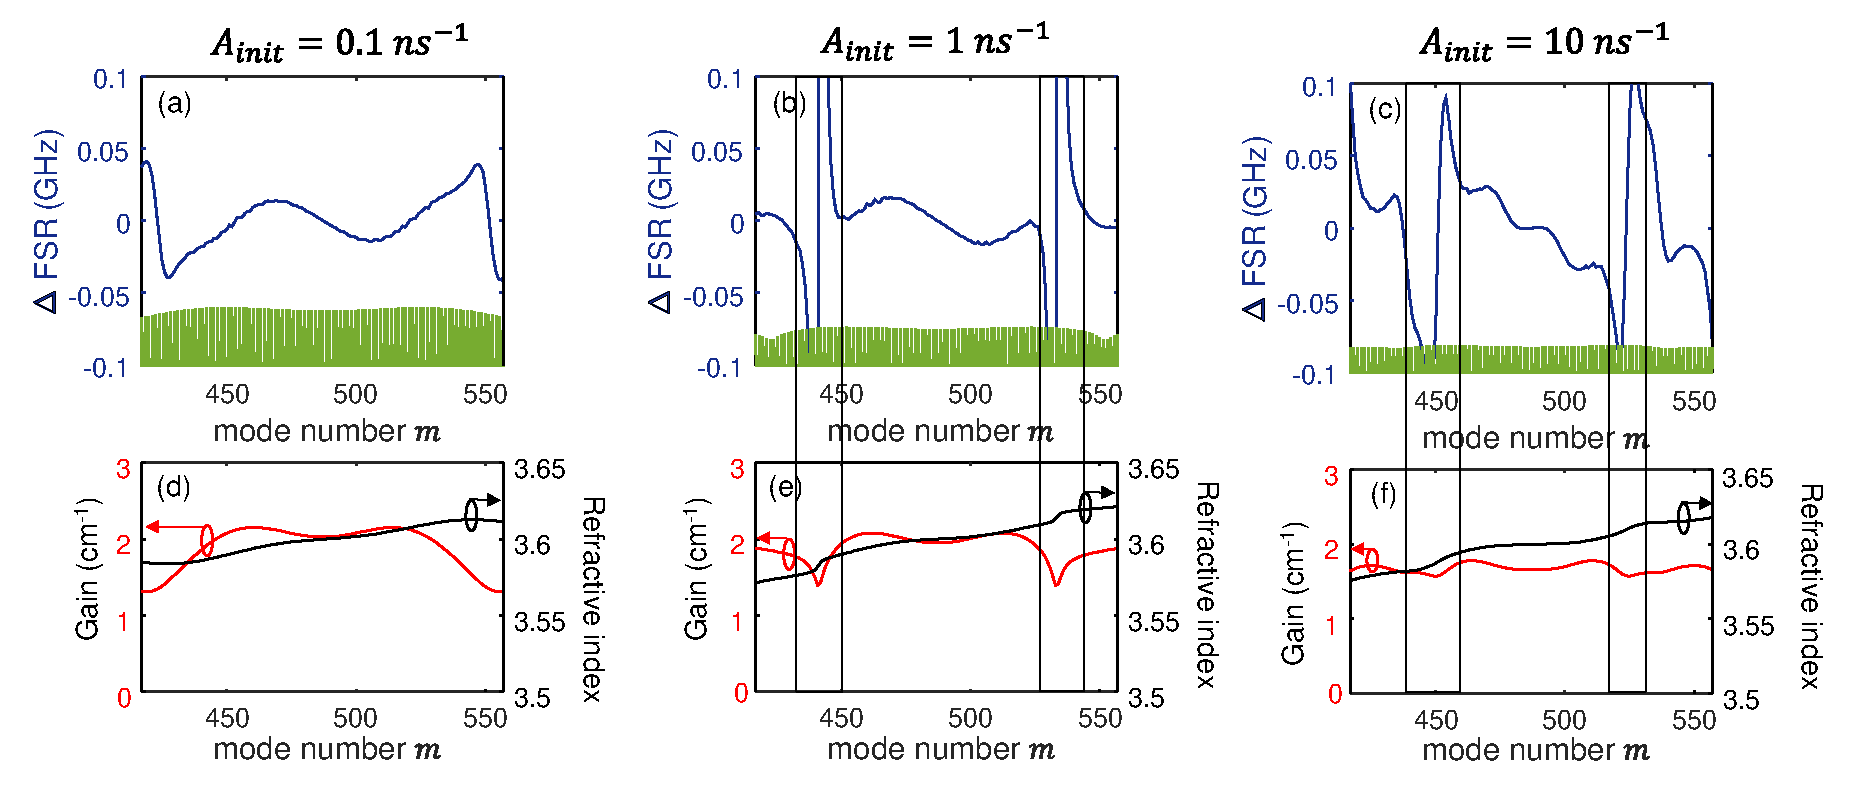
\includegraphics[width=0.85\textwidth]{IMGS/FSR_variation}
	\caption{Results from simulations of a numerical pump-probe experiment, performed with our model in Ref. \cite{petz2016}. (a), (b) and (c) display the variation of the free spectral range, as a function of the mode index $m$, for values of the pump  pulse amplitude, normalized to the Rabi-frequency, at 0.1 ns$^{-1}$, 1 ns$^{-1}$ and 10 ns$^{-1}$, respectively. For illustrative purposes we also plot the cavity modes (green lines), calculated via $f_m = m\times c/2Ln'(f_m)$, with amplitudes weighted by the normalized gain. (d), (e) and (f) Spectral gain (left y-axis) and the real part of the refractive index (right y-axis) as a function of the mode index $m$ and the pump pulse amplitude. All simulations were performed at value of the applied bias of 11 kV/cm, where the upper-lower laser level transition frequency was calculated at $f_0 = 4.05$ THz. The refractive index at $f_0$ was set to $n=3.6$ and the simulated cavity length was chosen as $L=5$ mm, giving a free spectral range $FSR(f_0) = 8.3$ GHz and a corresponding central mode index $m_0 = 487$.}	\label{fig:dispersion}
\end{figure*}

It is known that group velocity dispersion, i.e. frequency dependence of the refractive index, effects the equidistance of the Fabry-Perot modes, and thus hampers the formation of a comb. Direct estimation of the GVD of a device is difficult, as it has a strong dependence on the system parameters, waveguide design, as well as the power spectral density of the lasing modes (due to self- and cross- phase modulation effects) \cite{villares2016dispersion}. This also makes the theoretical treatment very challenging and therefore impedes the computer aided design of QCL frequency combs.

Again, we find that the Maxwell-Bloch equation provide us with a  suitable framework for the rigorous treatment of chromatic dispersion, as the density matrix equations intrinsically capture polarization effects, and thus the dispersion due to the optical gain. The model can be extended by the phenomenological inclusion of additional dispersive components, e.g. waveguide or bulk dispersion, and then the total system of equations numerically solved in the time-domain \cite{taflove2000computational}.

We restrict ourselves to modelling only dispersion due to optical resonances, i.e. gain dispersion, and in the following we perform several computational experiments to characterise it.

The general idea is to treat the gain medium of length $L$ as a nonlinear filter with some unknown transfer function $H(\omega)$. If were able to extract the magnitude and frequency response of this transfer function, we could use this information to infer the real and imaginary part of the refractive index. This can be done quite easily by simulating the passage of an unchirped pulse, e.g. a Gaussian with suitably chosen spectral width and amplitude, through the medium and recording the pulse at the output facet of the simulation region. The real power of this method lies in its universality, as it allows us to characterize the time-dependent behaviour of the system under different operating conditions, by simply varying the model parameters.

From basic laser theory~\cite{siegman1986lasers}, we know that a Fabry-Perot cavity of length $L$ will sustain longitudinal modes, determined by the relation 
$f_m = m \times c/2 L n'(f_m),$ where $m$ is some (large) integer, $f_m$ denotes the $m^{\text{th}}$ longitudinal mode, $c$ is the velocity of light in vacuum and $n'(f_m)$ is the value of the real part of the refractive index at that particular mode. The mode spacing at the $m^{\text{th}}$ longitudinal mode is also known as the free spectral range (FSR) and is given by $FSR(m)=f_{m+1}-f_{m}\approx c/2 L n'(f_m)$, which is generally index-dependent.

In free-running QCLs, due to their broadband nature and ultrafast carrier dynamics \cite{khurgin2014coherent}, there will be a strong competition between FWM and dispersion, the outcome of which will determine the free spectral range. This is because, while the former is an energy conserving process and thus tends to homogenize the mode spacing, the latter has a detrimental influence as it results in an FSR depending on frequency. It has been shown \cite{rosch2015octave} that at operation regimes where the different components of dispersion cancel each other out, or when special dispersion compensation mechanisms are employed \cite{burghoff2014terahertz}, four wave mixing can defeat intracavity dispersion, via the so called injection-locking effect, which then results in a broad comb spectrum. Generally, however, those comb regimes cover only a fraction of the whole dynamic range of the device and are usually limited to near-threshold operation. In fact, a clear explanation of why FWM looses to GVD at high pump intensities is somehow missing. It has been suggested \cite{rosch2015octave}, for example, that the appearance of more modes in the lasing spectra at higher values of the injection current, up to the boundaries of the spectral gain, increases the deteriorating effect of dispersion due to the higher values of the GVD coefficient at the periphery of the gain bandwidth. We would like to report that we observe another comb-degrading effect, which can be related to spatial hole burning-induced instabilities, and could be also one of the reasons for the breakdown of comb-like operation at high pump currents.  

First, we investigate in detail the frequency dependence of the refractive index, we the aid of the computational trick, outlined in the beginning of this section, when we vary the amplitude of the input pump pulse. In doing so, we can analyze the net effect of different intensity-dependent phenomena, such as gain saturation and also self and cross-phase modulation, onto the system dynamics. 

For these simulations we analyze the the QCL of Ref. \cite{burghoff2014terahertz}, again by applying our model from Ref. \cite{petz2016}. At the assumed operating bias of 11 kV/cm we have calculated that the injector and the upper laser level (in the tight-binding approximation - see Fig. \ref{fig:basis}(a) ) are almost perfectly aligned. As we show in the appendix, this results in a symmetric gain comprised of two equally strong frequency lobes, one for each allowed transition from a delocalized state to the ground level. This time, we set the cavity length to $5$ mm and propagate the pump pule only once before post processing. Figure \ref{fig:dispersion} illustrates the results from this procedure when we vary the strength of this input pulse. The latter is chosen as an unchirped Gaussian, with intensity full-width at half maximum (FWHM) of $1$ ps,  corresponding to a FWHM bandwith of 440 GHz (from the time-bandwidth product), whereas the amplitude is normalized to the Rabi-frequency of the material. 

As a figure of merit for the effect of chromatic dispersion on the comb-spacing, we calculate the frequency dependent variation of the free spectral range \cite{herr2012universal} via $\Delta FSR(m) = (f_{m+1}-f_{m}) - (f_{m} - f_{m-1}) $.  Figures~\ref{fig:dispersion}(a)-\ref{fig:dispersion}(c) illustrate the dependence of $\Delta FSR$ upon the pump pulse intensity. We also plot, Figs.~\ref{fig:dispersion}(d), \ref{fig:dispersion}(e) and \ref{fig:dispersion}(f), the shapes of the calculated spectral gain and the real part of the refractive index. 

The plots in Fig. \ref{fig:dispersion}(a)-\ref{fig:dispersion}(f) show the large changes in $\Delta FSR$ upon gain saturation. This is due to the fact that casuality \cite{toll1956} imposes an intimate relationship between the real and imaginary parts of the refractive index, via the Kramers-Kronig relations.  In particular, we see from Figs.~\ref{fig:dispersion}(b)-(c) and \ref{fig:dispersion}(e)-(f), that if the gain saturation over the lasing spectrum is inhomogeneous, due to the dependence $\Delta FSR(m) \propto \partial^2 f_m/\partial m^2 $, we could also expect strong variation of the free spectral range and thus highly uneven mode spacing. This reveals to us that dispersion control is a highly non-trivial problem, deeply rooted in the laser dynamics ( e.g. the fluctuations in the mode intensities), which might explain the difficulties of designing a dispersion compensation mechanism which can be effective over a broad range of operating conditions.  

As mentioned in the previous section, spatial hole burning is directly related to amplitude and phase instabilities in QCLs due to the effective lowering of the RNGH-instability threshold, and therefore deserves a more detailed study.  A thorough analytical investigation of SHB was already performed in Ref. \cite{gordon2008multimode} via a linear stability analysis of the Maxwell-Bloch equations. The authors managed to show how, in the presence of spatial hole burning, a two level system with a gain recovery time $T_1$ and a dephasing time $T_2$, will experience parametric gain around the central resonance frequency with maximum value at $$\Omega_{max}^2 \approx \frac{1}{T_1} \sqrt{\frac{p-1}{3T_1T_2}},$$ where $p$ is the pump parameter and $p=1$ means that the laser is biased exactly at threshold. 

If we would like the peaks of the parametric gain to be well outside the gain full width at half maximum bandwidth, i.e.  $\Delta\nu_{FWHM}$, assuming for simplicity that $T_1 \approx T_2$, we could impose the condition 
$$
T_1 \ll T_1^{max} = \frac{1}{\Delta\nu_{FWHM}}\sqrt{\frac{p-1}{3}}.
$$
Thus for lasers with extremely fast gain recovery, spatial hole burning will not play a vital role and can be thus neglected. How fast should this gain recovery time be? Well, this obviously depends on the strength with which one pumps above threshold, but for value of $p=2$, for example, and a value of $\Delta\nu_{FWHM}\approx 2\pi\times 1$ THz, this yields $T_1^{max}\approx 0.06 $ps, which is unfortunately too fast to be realistic. 

Another method to get rid of SHB is by incorporating the gain medium into a ring cavity instead of a Fabry-Perot one. In Ref. [cite Belyanin's nature paper] it has been demonstrated that by integrating the active region into an external ring cavity leads to dramatic improvement of the quality of active mode-locking and consecutively the emission of short pulses by a mid-IR QCL, known to be infamously hard to mode-lock. A more accessible method of reducing SHB is by creating a cavity with asymmetric mirror reflectivities such that the outcoupling is much stronger at, for example, the right facet of the cavity than the left. In such a scenario, the intensity of the right to left propagating component of each mode will be much smaller than the one in the opposite direction, which will lead to effective suppresion of the interference term in Eq. (\ref{eq:interference-effect}) and thus reduction of the depth of the inversion grating in Fig. \ref{fig:shb_graph}. An example of the behaviour of such a device will be presented in the next section, together with a detailed investigation of the temporal evolution of the modal phases and amplitudes.

\section{Time-evolution of the multimode spectra in QC lasers. The birth and the death of a comb.}
\begin{figure*}[h!]
	\centering
	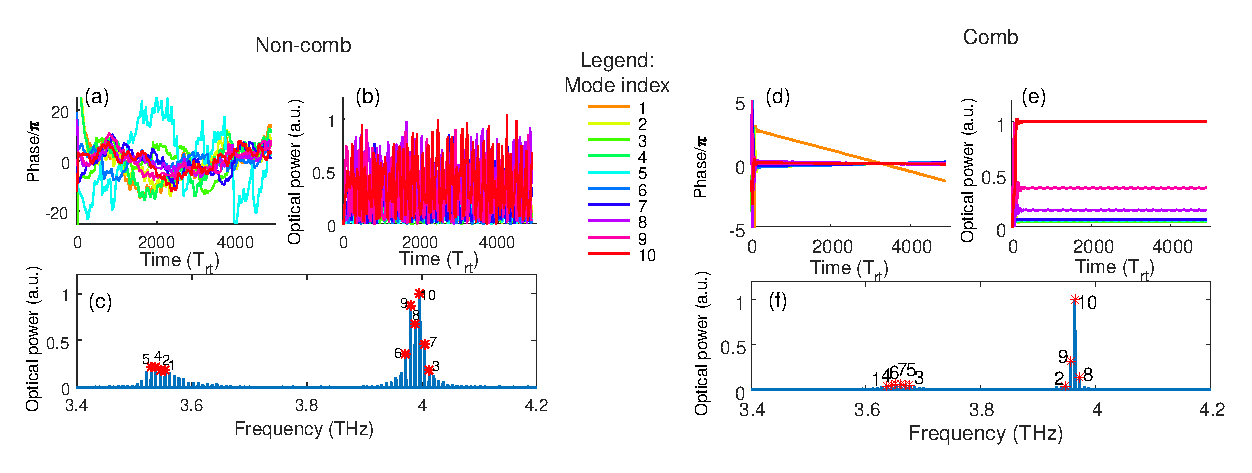
\includegraphics[width=0.85\textwidth]{IMGS/COMB_vs_NOCOMB1}
	\caption{Simulations of non-comb and comb regime of operation of a THz QC laser. These simulations are identical to the ones presented in Ref. \cite{petz2016}. (a) (b) and (c) modal phase, power and overall spectra of a dispersion uncompensated device. (d), (e) and (f) modal phase, power and overall spectra of a dispersion compensated device. The modal phases and powers were obtained via the short-time Fourier transform with a Hanning window function of duration 5 round trips (round tip time is approximately 120 ps) for a total simulation time of 5000 round trips, where the phases are presented after filtering out the constant linear drift with the aid of Matlab's "detrend" function. We plot the results for the 10 strongest modes in the corresponding spectra in c) and f). the locations of which are indicated by star-shaped markers.  The colour coding for each modes is presented in the legend (coloured version online)}	\label{fig:combnocomb1}
\end{figure*}

In the following we present results from long-time simulations of our device under study, i.e. the laser in Ref. \cite{burghoff2014terahertz},  for a self-starting free running configuration under different boundary conditions. First we reproduce our previously published simulation results \cite{petz2016}, however with an extended investigation of the time-dependence of the amplitude and phase of each lasing mode. This analysis reveals a clear trend in our simulations, which is that whenever spatial hole burning dominates the mode generation dynamics - the laser emits an unstable non-comb spectrum, and when SHB does not play an active role - a frequency comb. This also confirms our suggestions made in Sections \ref{sec:proliferation} and \ref{sec:combdegradation}, which underline the importance of the suppression of SHB for successful comb generation.

First, we consider comb and non-comb operation, reproduced by our simulations, when spatial hole burning plays an active role in the laser dynamics. Figure~\ref{fig:combnocomb1} displays the time-dependence phases, Figs.~\ref{fig:combnocomb1}(a) and \ref{fig:combnocomb1}(d), as well as the optical power at each mode for simulations with and without dispersion compensation. As mentioned in our past publication, the DCM mechanism was implemented via Fourier-transforming (in space) the intracavity field envelope and subtracting from the result a previously recorded nonlinear phase component. For more details on this technique we refer the reader to Ref.~\cite{petz2016}. 

A quick comparison of the different plots reveals a striking difference in the time-domain dynamics of both simulation scenarios. In Figs.~\ref{fig:combnocomb1}(a) and \ref{fig:combnocomb1}(b), demonstrating the non-comb operational regime, we observe chaotic fluctuation of both phase and amplitude without any noticeable regularity or tendency for convergence. In fact, it almost seems that all individual modes transiently switch on and off (due to the large oscillations in the modal power, noticeable in Fig.~\ref{fig:combnocomb1}(b)  at random intervals. This is namely a manifestation of multimode phase and amplitude instabilities discovered independently by Risken and Nummedal~\cite{risken1968self} as well as Graham and Haken~\cite{graham1968quantum}. As a comparison, whenever the laser operates as a comb, i.e. Figs.~\ref{fig:combnocomb1}(d) and \ref{fig:combnocomb1}(e), after several hundred round trips the longitudinal modes quickly converge to their steady state values with very little variation what so ever. Thus the modes are lasing constantly and are clearly phase-locked. It is worthwhile to note that we have observed the same effect not only for the top 10 strongest (in terms of stored power) modes, but in fact for all modes discernible on the optical power spectrum of Fig.~\ref{fig:combnocomb1}(f) (results not plotted here for clarity). This can be interpreted as that whenever dispersion compensation is efficient, four wave mixing completely overcomes spatial hole burning and stabilizes the laser output.
\begin{figure}[h!]
	\centering
	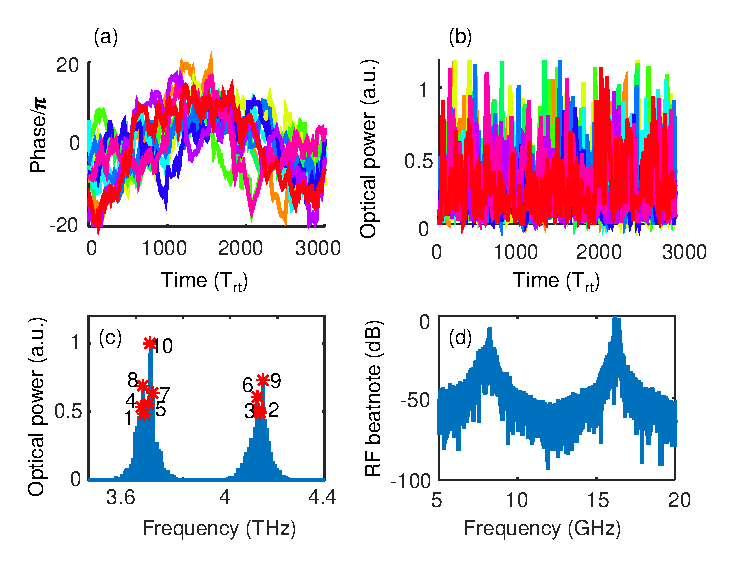
\includegraphics[width=0.45\textwidth]{IMGS/NOCOMB_NODISP}
	\caption{Simulation results for a free-running THz QCL, biased at injector-upper laser level resonance (11 kV/cm), where both the left and the right facet reflectivities were set at 100\%, in order to support a \emph{strong} spatial hole burning effect. (a) and (b) illustrate the modal phase and power of the top ten strongest lasing modes in the spectrum. (c) Optical power spectrum (normalized) and (d) radio-frequency (RF) beatnote of the simulated device. The modal characteristics, i.e. (a) and (b), were extracted using the short-time Fourier transform with a Hanning window of 5 round trips over a total simulation time of 3000 round trips. The colour coding is identical to Fig. \ref{fig:combnocomb1} (color online).}	\label{fig:NOCOMB_NODISP}
\end{figure}

To really nail down whether it is SHB that destroys the comb coherence we performed further simulations. First we simulated the same device, biased at 11 kV/cm, in a free-running regime of operation when both out-coupling mirror reflectivities were set to 100\%. This is the most favourable case for the formation of standing waves and thus the onset of SHB. Unsurprisingly, our simulation results revealed similar behaviour to the one in Figs.~\ref{fig:combnocomb1}(a)-\ref{fig:combnocomb1}(c), with chaotic variation of the spectral modes in Figs.~\ref{fig:NOCOMB_NODISP}(a)-\ref{fig:NOCOMB_NODISP}(b) and a multi-beatnote signal around $f_{rt} = 8.3$ GHz, Figs.~\ref{fig:NOCOMB_NODISP}(d). On the other hand, simulations with asymmetrically chosen out-coupling losses, where the left reflection coefficient was maintained at 100\% and the right one was set to 5\% show that the device acts as a comb, Figs. \ref{fig:COMB_NODISP}(a)-\ref{fig:COMB_NODISP}(d). Interstingly, in the second scenario we observe a strong and coherent beatnote only at the second harmonic of the linear cavity's round trip frequency $f_{rt}$. This is, of course, unsurprising since due to the unidirectionality of the field propagation the effective round trip time is halved, because only contributions from the forward propagating signal are sufficiently strong. Finally, we would like to stress on the fact that in both of those simulation scenarios no dispersion compensation mechanism was employed. 
\begin{figure}[h!]
	\centering
	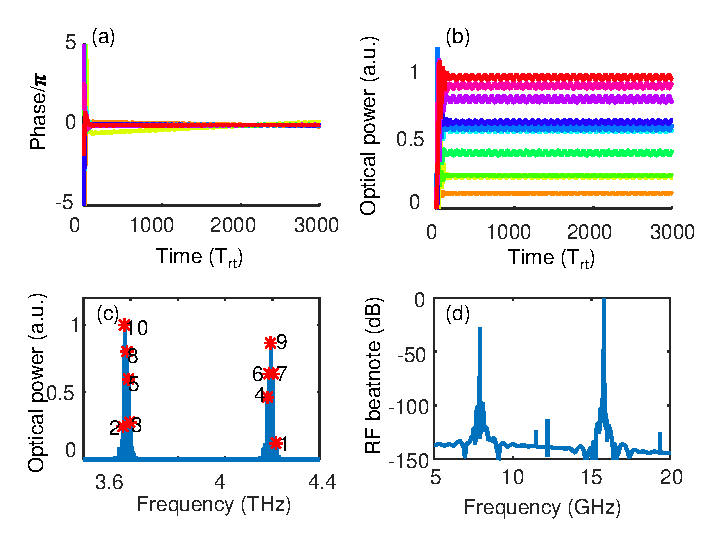
\includegraphics[width=0.45\textwidth]{IMGS/COMB_NODISP}
	\caption{Simulation results for the same configuration as in Fig. 
		\ref{fig:NOCOMB_NODISP}, with the difference that the right reflectivity coefficient was set to 5\%, whereas the left was maintained at 100\%, in order to support a \emph{weak} spatial hole burning effect. (a) and (b) depict the modal phase and power of the top 10 strongest modes, visible in the optical spectrum in (c). (c) Optical spectrum produced by the simulation with the top 10 modes indicated by red star-shape markers and corresponding mode index. (d) RF beatnote, produced by the simulation.}	\label{fig:COMB_NODISP}
\end{figure}
\section{Conclusion}
TODO finish up the conclusion -->

We have presented a theoretical model suitable for the simulation of THz QCLs in comb and non-comb regimes of operation, based on the full numerical solution of the Maxwell-Bloch equations in rotating wave approximation. We have shown that our approach correctly captures the complicated dynamics between four wave mixing, coherent tunneling and spectral gain splitting, group velocity dispersion, as well as spatial hole burning, as it delivers simulation results in good agreement with experimental data. We have used this model to characterize the spectral gain profile, the group velocity dispersion and to interplay between FWM and spatial hole burning (SHB) as dominant comb proliferation mechanisms. <-- TODO finish up the conclusion



\appendix
The fact that the original system's Hamiltonian is non-diagonal in the tight binding basis, introduces a new set of eigenstates, the so called delocalized basis states $\ket{+}$ and $\ket{-}$, both of which are radiatively coupled to the ground state $\ket{2}$. One can obtain the new set of eigenstates from the tight binding states via the unitary transform
\begin{align}
\label{eq:dressedstates}
\Ket{+} &= \cos\theta \Ket{1'} - \sin\theta \Ket{3}, \nonumber \\
\Ket{-} &= \sin\theta \Ket{1'} + \cos\theta \Ket{3}.
\end{align}
The eigenenergies are given by
\begin{equation}
E_\pm =\hslash \omega_{\pm} =\hbar(\omega_{32} +\epsilon/2) \pm \hbar \sqrt{\epsilon^2+4\Omega_{1'3}^2}/2,
\end{equation}
and the expansion coefficients, i.e. $\cos\theta$ and $\sin\theta$, are computed from  
$
\tan \theta = -2\Omega_{1'3}/[\epsilon+(\epsilon^2+4\Omega_{1'3}^2)^{1/2}].
$
From here, one can compute the magnitude of the ratio of the dipole matrix elements $d_{\pm 2} = \bra{\pm}\h z \ket{2}$, between the delocalized states and the ground state level $\ket{2}$, as $|d_{+2}|/|d_{-2}| \approx |\tan\theta|$. This allows us to examine the bias dependence of the dominant transition \cite{dupont2010simplified} as when $\epsilon >0$, $|\tan\theta|<1$ and thus the low frequency transition will have a higher dipole moment, whereas for $\epsilon < 0 $  it will be vice versa. In fact, from Eq. \ref{eq:dressedstates}, we can see that the strength of the dipole moment $d_{32}$ in the tight-binding approximation is related to $d_{\pm2}$ via the quadratic relation
\begin{equation}
d_{32}^2 =d_{+2}^2+d_{-2}^2.
\end{equation}  
An interesting case to consider is when the detuning from injector-upper laser level resonance satisfies $\epsilon \ll 1 $ meV. In such a case, both transitions will be equally likely and thus the laser ought to have a symmetrically shaped spectral gain.    





% References <- adhere to respective journal style 
\bibliographystyle{IEEEtran}
\bibliography{D:/docs/MAIN-PROJECTS/PAPERS/literature/bib_resources}


\end{document} 
